\documentclass[notheorems, hyperref={backref}]{beamer}

%% KEY LINES IN THIS TEX FILE %% (enter line number+gg to go)

%
% LOCAL FONT DEFINITIONS -- need to come first
%
%\usepackage{mathpazo}
\usepackage{libertine}
\usepackage[libertine]{newtxmath}
\usefonttheme[onlymath]{serif}

%
% STANDARD PREAMBLE
%
%
% PACKAGES
%

\usepackage[T1]{fontenc}
% This uses 8-bit font encoding (with 256 glyphs) instead of the default 7-bit font encoding (with 128 glyphs). For example, with this option ö is a single glyph in the font, whereas on the 7-bit font encoding the font ö is made by adding an accent to the existing glyph o. A bad consequence of not using this package is that you cannot properly copy-paste such words form the output pdf file. Also, for some reason, funny stuff happens with |, < and > in text.

% Some people suggest to load fontenc before inputenc, most agree that it does not matter.

\usepackage[utf8]{inputenc}
% When you type ä in an editor set up for utf8, the machine stores the character number 228. When TeX reads the file it finds the character number 228 and the macros of inputenc transform this into \"a. Finally fontenc does its thing and transforms this into the command print character 228 (otherwise the two things would be printed separatedly as explained in fontenc).

\usepackage[UKenglish]{babel}
% To manage culturally determined typographical and similar rules, in this case for british english. Some people suggest to load babel after fontenc to avoid warnings, although most agree that it does not matter.

\usepackage{mathtools}
% Loads the amsmath package (\usepackage{amsmath}: miscellaneous improvements such as the commands \DeclareMathOperator and \text). It fixes some quirks it has and adds some useful settings, symbols and environments. It improves the aesthetics as well.

\usepackage{amssymb}
% Extended symbol collection, e.g. \Cap and \Cup. More importantly: the \mathbb command! It loads the amsfonts package (\usepackage{amsfonts}: fraktur letters, bold Greek letters...), so we do not need to include it in the preamble anymore.

\usepackage{mathrsfs}
% Font package (only supports upper case letters).

\usepackage{enumitem}
% To control the layout of enumerate, itemize and description. It supersedes the enumerate package.

\usepackage{tikz-cd}
% To draw commutative diagrams.
\usetikzlibrary{decorations.markings}
% For open and closed immersions.

\usepackage{graphicx}
% An extension of the graphics package, with optional arguments for the \includegraphics command.

\usepackage{todonotes}
% To write to do notes use the command \todo.

% \usepackage{xcolor}
% To write in colors.
% Already loaded by beamer class.

\usepackage{mathdots}
% To draw diagonal dots.

\usepackage{marginnote}
% To write on margins.

\usepackage{manfnt}
% To draw dangerous bent symbol.

\usepackage{float}
% Improved interface for floating objects such as figures and tables, introducing for example the H modifier to force the position of a float in the page or the boxed float. Should be loaded before hyperref.

% \usepackage[backref]{hyperref}
% To handle cross-referencing and produce hypertext links in the document. It should be loaded last (with few exceptions), because it redefines many LaTeX commands.
% The backref option inserts links on each bibliography entry to the pages in which the citation was used.
%% The hidelinks option removes colors and boxes around links, but the links remain clickable. On firefox the links are even highlighted when the mouse pointer passes over them.
% \renewcommand{\backref}[1]{$\uparrow$~#1}
% Adds an upwards arrow before referencing to the pages in which the citations appear.
% Already loaded by beamer class.

\usepackage[noabbrev]{cleveref}
% Enhances cross-referencing features, e.g. to reference to a theorem and automatically include the word theorem.
% No abbreviature option to write figure instead of fig. etc.

% Open and closed immersion arrows.
\makeatletter
\tikzcdset{
open/.code={\tikzcdset{hook, circled};},
closed/.code={\tikzcdset{hook, slashed};},
circled/.code={\tikzcdset{markwith={\draw (0,0) circle (.375ex);}};},
slashed/.code={\tikzcdset{markwith={\draw[-] (-.4ex,-.4ex) -- (.4ex,.4ex);}};},
markwith/.code={
\pgfutil@ifundefined{tikz@library@decorations.markings@loaded}%
{\pgfutil@packageerror{tikz-cd}{You need to say %
\string\usetikzlibrary{decorations.markings} to use arrow with markings}{}}{}%
\pgfkeysalso{/tikz/postaction={/tikz/decorate,
/tikz/decoration={
markings,
mark = at position 0.5 with
{#1}}}}},
}
\makeatother

% Custom colors
\definecolor{darkgreen}{RGB}{0,75,0}
\definecolor{darkblue}{RGB}{0,0,75}
\definecolor{darkred}{RGB}{75,0,0}
\definecolor{linkred}{rgb}{0.7,0.2,0.2}
\definecolor{linkblue}{rgb}{0,0.2,0.6}

% Limit table of contents to section titles
\setcounter{tocdepth}{1}

% Sloppy formatting -- often looks better
\sloppy

%
% FONT DEFINTIONS
%

% Script Font used for sheaves
\DeclareFontFamily{OMS}{rsfs}{\skewchar\font'60}
\DeclareFontShape{OMS}{rsfs}{m}{n}{<-5>rsfs5 <5-7>rsfs7 <7->rsfs10 }{}
\DeclareSymbolFont{rsfs}{OMS}{rsfs}{m}{n}
\DeclareSymbolFontAlphabet{\scr}{rsfs}
\DeclareSymbolFontAlphabet{\scr}{rsfs}

% Sheaves
\newcommand{\sA}{\scr{A}}
\newcommand{\sB}{\scr{B}}
\newcommand{\sC}{\scr{C}}
\newcommand{\sD}{\scr{D}}
\newcommand{\E}{\scr{E}} % Exception (Vector bundles)
\newcommand{\F}{\scr{F}} % Exception (Coherent sheaves)
\newcommand{\G}{\scr{G}} % Exception (Coherent sheaves)
\newcommand{\sH}{\scr{H}}
\renewcommand{\hom}{\scr{H}\negthinspace om} % Exception (Hom-sheaf)
\newcommand{\I}{\scr{I}} % Exception (Ideal sheaves)
\newcommand{\sJ}{\scr{J}}
\newcommand{\sK}{\scr{K}}
\renewcommand{\L}{\scr{L}} % Exception (Line bundles)
\newcommand{\M}{\scr{M}} % Exception (Line bundles)
\newcommand{\sN}{\scr{N}}
\renewcommand{\O}{\scr{O}} % Exception (Structure sheaf)
\newcommand{\sP}{\scr{P}}
\newcommand{\sQ}{\scr{Q}}
\newcommand{\sR}{\scr{R}}
\newcommand{\sS}{\scr{S}}
\newcommand{\sT}{\scr{T}}
\newcommand{\sU}{\scr{U}}
\newcommand{\sV}{\scr{V}}
\newcommand{\sW}{\scr{W}}
\newcommand{\w}{\omega} % Addition (Canonical sheaf)
\newcommand{\sX}{\scr{X}}
\newcommand{\sY}{\scr{Y}}
\newcommand{\sZ}{\scr{Z}}

% Mathcal fonts
\newcommand{\calA}{\mathcal{A}}
\newcommand{\calB}{\mathcal{B}}
\newcommand{\calC}{\mathcal{C}}
\newcommand{\calD}{\mathcal{D}}
\newcommand{\calE}{\mathcal{E}}
\newcommand{\calF}{\mathcal{F}}
\newcommand{\calG}{\mathcal{G}}
\newcommand{\calH}{\mathcal{H}}
\newcommand{\calI}{\mathcal{I}}
\newcommand{\calJ}{\mathcal{J}}
\newcommand{\calK}{\mathcal{K}}
\newcommand{\calL}{\mathcal{L}}
\newcommand{\calM}{\mathcal{M}}
\newcommand{\calN}{\mathcal{N}}
\newcommand{\calO}{\mathcal{O}}
\newcommand{\calP}{\mathcal{P}}
\newcommand{\calQ}{\mathcal{Q}}
\newcommand{\calR}{\mathcal{R}}
\newcommand{\calS}{\mathcal{S}}
\newcommand{\calT}{\mathcal{T}}
\newcommand{\U}{\mathcal{U}} % Exception (Open covers)
\newcommand{\calV}{\mathcal{V}}
\newcommand{\calW}{\mathcal{W}}
\newcommand{\X}{\mathcal{X}} % Exception (Families of varieties)
\newcommand{\Y}{\mathcal{Y}} % Exception (Families of varieties)
\newcommand{\calZ}{\mathcal{Z}}

% Blackboard Bold Symbols
\newcommand{\A}{\mathbb{A}} % Exception (Affine space)
\newcommand{\bbB}{\mathbb{B}}
\newcommand{\C}{\mathbb{C}} % Exception (Complex numbers)
\newcommand{\bbD}{\mathbb{D}}
\newcommand{\bbE}{\mathbb{E}}
\newcommand{\bbF}{\mathbb{F}}
\newcommand{\bbG}{\mathbb{G}}
\newcommand{\Gm}{\mathbb{G}_{\mathrm{m}}} % Addition (Punctured affine line)
\newcommand{\bbH}{\mathbb{H}}
\newcommand{\bbI}{\mathbb{I}}
\newcommand{\bbJ}{\mathbb{J}}
\newcommand{\bbK}{\mathbb{K}}
\renewcommand{\k}{\Bbbk} % Addition (Field)
\newcommand{\bbL}{\mathbb{L}}
\newcommand{\bbM}{\mathbb{M}}
\newcommand{\N}{\mathbb{N}} % Exception (Natural numbers)
\newcommand{\bbO}{\mathbb{O}}
\renewcommand{\P}{\mathbb{P}} % Exception (Projective space)
\newcommand{\Q}{\mathbb{Q}} % Exception (Rational numbers)
\newcommand{\R}{\mathbb{R}} % Exception (Real numbers)
\newcommand{\bbS}{\mathbb{S}}
\newcommand{\bbT}{\mathbb{T}}
\newcommand{\bbU}{\mathbb{U}}
\newcommand{\V}{\mathbb{V}} % Exception (Geometric vector bundle)
\newcommand{\bbW}{\mathbb{W}}
\newcommand{\bbX}{\mathbb{X}}
\newcommand{\bbY}{\mathbb{Y}}
\newcommand{\Z}{\mathbb{Z}} % Exception (Integers)

% Boldfont (categories)
\newcommand{\bfA}{\mathbf{A}}
\newcommand{\Ab}{\mathbf{Ab}}
\newcommand{\bfB}{\mathbf{B}}
\newcommand{\bfC}{\mathbf{C}}
\newcommand{\Cat}{\mathbf{Cat}} % Addition (Categories)
\newcommand{\Coh}{\mathbf{Coh}} % Addition (Coherent sheaves)
\newcommand{\D}{\mathbf{D}} % Exception (Derived category)
\newcommand{\Db}{\mathbf{D}^{\mathrm{b}}} % Addition (Bounded derived category)
\newcommand{\bfE}{\mathbf{E}}
\newcommand{\bfF}{\mathbf{F}}
\newcommand{\bfG}{\mathbf{G}}
\newcommand{\bfH}{\mathbf{H}}
\newcommand{\bfI}{\mathbf{I}}
\newcommand{\bfJ}{\mathbf{J}}
\newcommand{\K}{\mathbf{K}} % Exception (Homotopy category)
\newcommand{\bfL}{\mathbf{L}}
\newcommand{\bfM}{\mathbf{M}}
\newcommand{\Mod}{\mathbf{Mod}} % Addition (Modules)
\newcommand{\bfN}{\mathbf{N}}
\newcommand{\bfO}{\mathbf{O}}
\newcommand{\bfP}{\mathbf{P}}
\newcommand{\PSh}{\mathbf{PSh}} % Addition (Presheaves)
\newcommand{\bfQ}{\mathbf{Q}}
\newcommand{\QCoh}{\mathbf{QCoh}} % Addition (Quasi-coherent sheaves)
\newcommand{\bfR}{\mathbf{R}}
\newcommand{\bfS}{\mathbf{S}}
\newcommand{\Set}{\mathbf{Set}} % Addition (Sets)
\newcommand{\Sh}{\mathbf{Sh}} % Addition (Sheaves)
\newcommand{\bfT}{\mathbf{T}}
\renewcommand{\Top}{\mathbf{Top}} % Addition (Topological spaces)
\newcommand{\bfU}{\mathbf{U}}
\newcommand{\bfV}{\mathbf{V}}
\renewcommand{\Vec}{\mathbf{Vec}} % Addition (Vector bundles)
\newcommand{\bfW}{\mathbf{W}}
\newcommand{\bfX}{\mathbf{X}}
\newcommand{\bfY}{\mathbf{Y}}
\newcommand{\bfZ}{\mathbf{Z}}

% Mathfrak for ideals
\renewcommand{\a}{\mathfrak{a}}
\renewcommand{\b}{\mathfrak{b}}
\renewcommand{\c}{\mathfrak{c}}
\renewcommand{\d}{\mathfrak{d}}
\newcommand{\e}{\mathfrak{e}}
\newcommand{\m}{\mathfrak{m}}
\newcommand{\n}{\mathfrak{n}}

% Custom theorem styles (empty fields take default values)
\newtheoremstyle{darkgreentheorem}% name of the style
{}% measure of space to leave above the theorem. E.g.: 3pt
{}% measure of space to leave below the theorem. E.g.: 3pt
{\itshape}% name of font to use in the body of the theorem
{}% measure of space to indent
{\color{darkgreen}\bfseries}% name of head font
{}% punctuation between head and body
{ }% space after theorem head; " " = normal interword space
{}% Manually specify head
\newtheoremstyle{darkbluedefinition}
{}{}{}{}{\color{darkblue}\bfseries}{}{ }{}
\newtheoremstyle{darkredexample}
{}{}{}{}{\color{darkred}\bfseries}{}{ }{}



\allowdisplaybreaks

% Extra packages
\usepackage{relsize}

% TIkzlibraries
\usetikzlibrary{decorations.pathmorphing}

%
% ABOUT FONT DEFINTIONS IN THE PREAMBLE
%
% Mathscr for sheaves use \sA, where A can be any letter. Exceptions and additions:
% % \E (vector bundles)
% % \F (coherent sheaves)
% % \G (coherent sheaves)
% % \hom (sheaf hom)
% % \I (ideal sheaves)
% % \L (line bundles)
% % \M (line bundles)
% % \O (structure sheaf)
% % \w (canonical sheaf)
%
% Mathcal use \calA. Exceptions and additions:
% % \U (open cover)
% % \X (families of varieties)
% % \Y (families of varieties)
%
% Mathbb use \bbA. Exceptions and additions:
% % \A (affine space)
% % \C (complex numbers)
% % \Gm (puctured affine line)
% % \k (field)
% % \N (natural numbers)
% % \P (projective space)
% % \Q (rational numbers)
% % \R (real numbers)
% % \V (geometric vector bundle)
% % \Z (integers)
%
% Boldfont for categories use \bfA. Additions:
% % \Cat (categories)
% % \Coh (coherent sheaves)
% % \D (derived category)
% % \Db (bounded derived category)
% % \K (homotopy category)
% % \Mod (modules)
% % \PSh (presheaves)
% % \QCoh (quasi-coherent sheaves)
% % \Set (sets)
% % \Sh (sheaves)
% % \Top (topological spaces)
% % \Vec (vector bundles)
%
% Mathfrak for ideals
% % From \a to \e
% % \m and \n for maximal ideals

%
% THEOREM ENVIRONMENTS
%
\setbeamertemplate{theorems}[numbered]
\newtheorem*{thm}{Theorem}
\newtheorem{exe}{Exercise}

%
% THEOREM CROSS-REFERENCING
%
\crefname{thm}{theorem}{theorems}
\Crefname{thm}{Theorem}{Theorems}
\crefname{lm}{lemma}{lemmas}
\Crefname{lm}{Lemma}{Lemmas}
\crefname{prop}{proposition}{propositions}
\Crefname{prop}{Proposition}{Propositions}
\crefname{cor}{corollary}{corollaries}
\Crefname{cor}{Corollary}{Corollaries}
\crefname{conj}{conjecture}{conjectures}
\Crefname{conj}{Conjecture}{Conjectures}
\crefname{defn}{definition}{definitions}
\Crefname{defn}{Definition}{Definitions}
\crefname{exa}{example}{examples}
\Crefname{exa}{Example}{Examples}
\crefname{rem}{remark}{remarks}
\Crefname{rem}{Remark}{Remarks}
\crefname{nota}{notation}{notations}
\Crefname{nota}{Notation}{Notations}
\crefname{fact}{fact}{facts}
\Crefname{fact}{Fact}{Facts}
\crefname{q}{question}{questions}
\Crefname{q}{Question}{Questions}
\crefname{pbl}{problem}{problems}
\Crefname{pbl}{Problem}{Problems}

%
% MATH OPERATORS
%
\DeclareMathOperator{\Hom}{Hom}
\DeclareMathOperator{\Fib}{Fib}
\DeclareMathOperator{\id}{id}
\DeclareMathOperator{\Aut}{Aut}

%
% OTHER COMMANDS
%
\newcommand{\ot}{\otimes}
\newcommand{\op}{\oplus}
\newcommand{\Cov}{\mathbf{Cov}}
\newcommand{\act}{\mbox{ }\rotatebox[origin=c]{-120}{$\circlearrowright$}}

%
% TITLE PAGE INFORMATION
%
\title[Basics of monodromy]{Basics of Monodromy}
\author{Pedro Núñez}
\institute{Basic Notions --- University of Freiburg}
\date{14th May 2020}
 
%
% LINKS AND PDF OPTIONS
%
\makeatletter
\hypersetup{
  %pdfauthor={\authors},
  pdftitle={\@title},
  %pdfsubject={\@subjclass},
  %pdfkeywords={\@keywords},
  %pdfstartview={Fit},
  %pdfpagelayout={TwoColumnRight},
  %pdfpagemode={UseOutlines},
  bookmarks,
  colorlinks,
  linkcolor=linkblue,
  citecolor=linkred,
  urlcolor=linkred}
\makeatother

% Table of contents
\setbeamertemplate{section in toc}[sections numbered]

% Add table of contents at the beginning of each section
\AtBeginSection[]
{
    \begin{frame}
	\frametitle{Table of Contents}
	\tableofcontents[currentsection]
    \end{frame}
}
\usecolortheme{orchid}
 
\begin{document}
 
\frame{\titlepage}

\section{Introduction}
\begin{frame}
    \frametitle{Motivating example --- A multi-valued function}
    Consider $z=re^{\theta i}\mapsto z^{2}=r^{2}e^{2\theta i}$ on $\C$.
    Local inverse on $\C^{\times}$:
    \[ z=re^{\theta i} \mapsto \sqrt{z}=\sqrt{r}e^{\frac{\theta}{2}i}. \]
    \pause

    \textbf{Ambiguity:} the previous expression is not well defined, as
    \[ re^{\theta i}=re^{(\theta+2\pi)i}\mapsto \sqrt{r}e^{\frac{\theta}{2}i}\neq \sqrt{r}e^{\left(\frac{\theta}{2}+\pi\right)i}. \]
    \pause

    Let $z_{0}\in \C^{\times}$ and pick one value for $\sqrt{z_{0}}$.
    Let $\gamma\colon [0,1]\to \C^{\times}$ be a path with $\gamma(0)=z_{0}$.
    Then the chosen $\sqrt{z_{0}}$ determines uniquely a value of $\sqrt{\gamma(t)}$ for all $t\in [0,1]$, because we want $z\mapsto \sqrt{z}$ to be continuous.
\end{frame}
 
\begin{frame}
    \frametitle{The Monodromy Theorem}
    \begin{thm}[Weierstraß]
	Analytic continuation along a path only depends on the path up to homotopy.
    \end{thm}
    \pause
    \vspace{2em}
    In particular, if we walk around a simply connected space, then the analytic continuation is single-valued everywhere.
    \pause
    \vspace{2em}
    Hence:
    
    \textbf{``monodromy''}, \textit{mónos} (alone, only, single) and \textit{drómos} (running).
\end{frame}

\begin{frame}
    \frametitle{Polydromy, a.k.a.~lack of monodromy}
    Let's go back to our example $z\mapsto \sqrt{z}$ on $\C^{\times}$.
    \pause

    Pick a value of $\sqrt{1}$, say $1$ itself, and let $\gamma\colon [0,1]\to \C^{\times}$ be a loop at $1$ around $0$.
    Extend $\sqrt{z}$ along $\gamma$ as before.
    \pause
    \begin{figure}[htp]
	\centering
	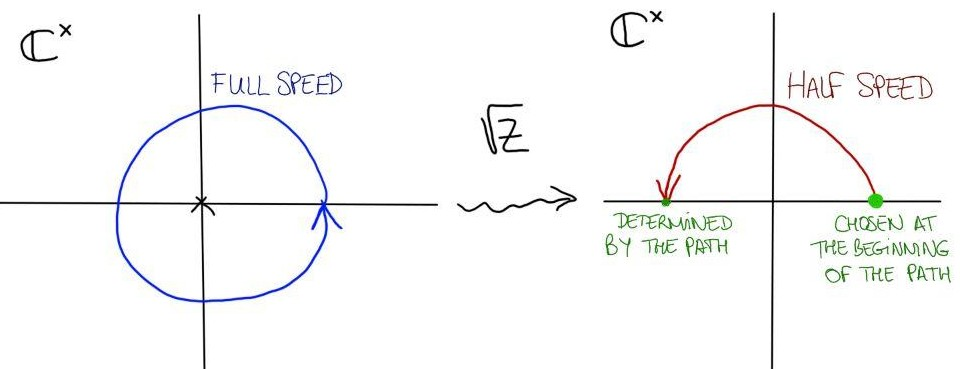
\includegraphics[scale=.3]{pictures/root.jpg}
	\caption{After the loop we arrive at $-1$, the other possible value of $\sqrt{1}$.}
    \end{figure}
\end{frame}

\begin{frame}
    \frametitle{Why are we then talking about monodromy?}
    The Monodromy Theorem became so famous that people kept using the word ``monodromy'' to talk about polydromy\footnote{Frans Oort gave this explanation to Fabrizio Catanese.}.
    \pause
    \begin{figure}[htp]
	\centering
	
\includegraphics[scale=.3]{pictures/RedHerring.png}
	\caption{This is an example of \href{https://ncatlab.org/nlab/show/red+herring+principle}{mathematical red herring principle}.}
    \end{figure}
    \pause
    \setcounter{exe}{-1}
    \begin{exe}
	This is the second red herring that appeared in this talk so far.

	Can you spot the first one?
    \end{exe}
\end{frame}

\begin{frame}
    \frametitle{Goal: understand polydromy}
    The Monodromy Theorem implies that $\pi_{1}(\C^{\times},z_{0})$ acts on the different possible values of $\sqrt{z_{0}}$.
    \pause

    The goal of this talk is to generalize this situation as follows:
    \pause
    \begin{enumerate}[label=\textbullet]
	\setlength\itemsep{1em}
	\item As we move $z$ in $\C^{\times}$, the possible values of $\sqrt{z}$ form a nice \textbf{covering space} of $\C^{\times}$.
	\pause
	\item If $p\colon Y\to X$ is a nice covering space, then $\pi_{1}(X,x)$ acts naturally on $p^{-1}(x)$.
	    This is the \textbf{monodromy action}.
	\pause
    \item We can recover the covering space from the monodromy action.
	\pause
    \item If the fibres of $p$ carry a natural vector space structure, then one can use the tools of \textbf{representation theory} to study polydromy.
	\pause
	This happens both naturally (e.g.~when solving differential equations on a complex domain) and artificially (e.g.~replacing the fibres by their cohomology groups).
    \end{enumerate}
\end{frame}

\section{Galois correspondence}
\begin{frame}
    \frametitle{Covering spaces}
    Let $X$ be a topological space.
    \pause
    \begin{enumerate}[label=\textbullet]
	\setlength\itemsep{1em}
	\item The category of \textit{spaces over $X$} has for objects (continuous) maps $p\colon Y\to X$ and for morphisms commutative triangles
	    \begin{center}
		\begin{tikzcd}[ampersand replacement=\&]
		    Y_{1}\arrow[swap]{dr}{p_{1}}\arrow{rr}{f} \& \& Y_{2}\arrow{dl}{p_{2}} \\
		    \& X \& 
		\end{tikzcd}
	    \end{center}
	    \pause
	\item A map $p\colon Y\to X$ has property $\mathbf{P}$ \textit{locally on $X$} if every point $x\in X$ has an open neighbourhood $x\in U\subseteq X$ such that $\mathbf{P}$ is true for $p|_{p^{-1}(U)}\colon p^{-1}(U)\to U$.
	    \pause
	\item $p\colon Y\to X$ is a \textit{covering space} if locally on $X$ it is isomorphic to a projection $X\times F\to X$ for some discrete space $F$.
    \end{enumerate}
\end{frame}

%\begin{frame}
%    \frametitle{Examples}
%    \begin{enumerate}[label=\textbullet]
%	\setlength\itemsep{1em}
%	\item Let $F$ be a discrete space.
%	    Then the projection $X\times F\to X$ is a cover, called a \textit{trivial cover} of $X$.
%	    \pause
%	\item Let $\Z$ act on $\R$ by translation $n\cdot x:=x+n$.
%	    Then the quotient map $\R\to \R/\Z=S^{1}$ is a cover.
%	    Could it be a trivial cover?
%	\item Consider again the map $z\mapsto z^{2}$.
%	    This does not define a cover over $\C$, because $0$ is a \textit{branching point}.
%	    But it does define a cover over $\C^{\times}$.
%    \end{enumerate}
%    \pause
%    \begin{exe}
%	A (continuous) group action $G\act Y$ is called \textit{even} if each $y\in Y$ has an open neighbourhood $y\in V\subseteq Y$ such that the sets $gV$ are pairwise disjoint for all $g\in G$.
%
%	If $G\act Y$ is even, then $p_{G}\colon Y\to G\backslash Y$ is a covering.
%    \end{exe}
%\end{frame}

\begin{frame}
    \frametitle{Maps into covering spaces} 
    \begin{figure}[htp] 
	\centering
	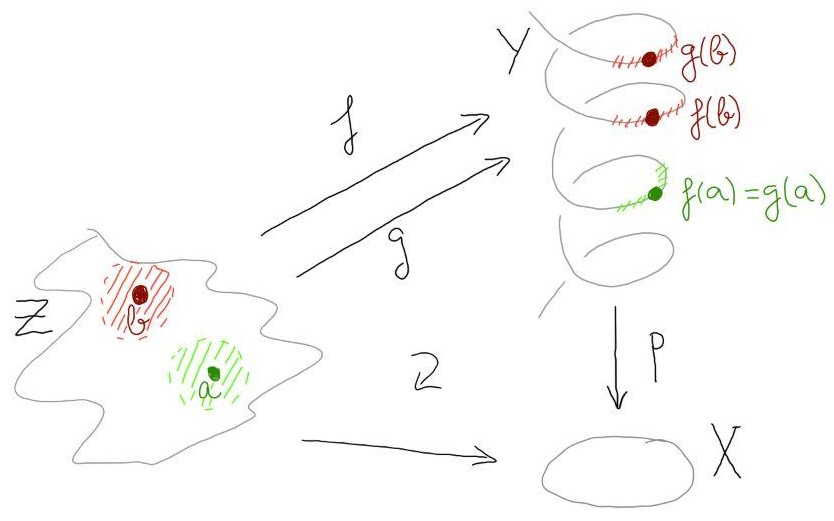
\includegraphics[scale=.25]{pictures/lemma.jpg}
	\caption{The set $\{z\in Z\mid f(z)=g(z)\}$ is open and closed, so if $Z$ is connected and $f$ and $g$ agree on a single point, then they agree in all of $Z$.}
    \end{figure}
    \pause
    In particular, if $p\colon Y\to X$ is a connected cover and $\phi\in \Aut(Y\mid X)$ fixes a point, then $\phi=\id_{Y}$.
\end{frame}

%\begin{frame}
%    \frametitle{Some more consequences}
%    \begin{enumerate}[label=\textbullet]
%	\setlength\itemsep{1em}
%	\item If $p\colon Y\to X$ is a connected cover, then $\Aut(Y\mid X)\act Y$ is even.
%	    \pause
%	\item We saw earlier that if $G\act Y$ is even, then $Y\to G\backslash Y$ is a cover.
%	    Suppose $Y$ is connected.
%	    \pause
%	    Define a group homomorphism:
%	    \begin{align*}
%		G & \longrightarrow \Aut(Y\mid G\backslash Y) \\
%		g & \longmapsto (y\mapsto g\cdot y)
%	    \end{align*}
%	    \pause
%	    \begin{enumerate}[label=$\circ$]
%		\item Since $G\act Y$ is even, $G\to \Aut(Y\mid G\backslash Y)$ is injective.
%		\pause
%
%		\item For $\phi\in \Aut(Y\mid G\backslash Y)$ and $y_{0}\in Y$, there is $g\in G$ with $\phi(y_{0})=g\cdot y_{0}$, because the fires are orbits and $\phi$ preservves fibres.
%		\pause
%		Since $Y$ is connected, $\phi(y)=g\cdot y$ for all $y\in Y$.
%	    \end{enumerate}
%    \end{enumerate}
%\end{frame}

\begin{frame}
    \frametitle{Galois correspondence [$X$ locally connected]}
    A connected cover $p\colon Y\to X$ is called \textit{Galois} if $X=\Aut(Y\mid X)\backslash Y$;
    \pause

    equivalently, if $\Aut(Y\mid X)$ acts transitively on each fibre.
    \pause

    \begin{thm}[{\cite[Theorem 2.2.10]{sza08}}]
	Let $p\colon Y\to X$ be a Galois cover.
	Then there is a bijection
	\begin{align*}
	    \left\{ \begin{matrix*}
		\mathrm{ Subgroups } \\
	    0\subseteq H\subseteq \Aut(Y\mid X)
	    \end{matrix*} \right\} & \leftrightarrow \left\{ \begin{matrix*}
		\mathrm{Connected} \\
		\mathrm{intermediate} \\
		\mathrm{covers}
	    \end{matrix*} 
	    \quad
	    \begin{tikzcd}[ampersand replacement=\&]
		Z\arrow[swap]{d}{q} \& Y\arrow{dl}{p}\arrow[dashed, swap]{l}{\exists} \\
		X \&
	    \end{tikzcd}
	    \right\} \\
	    H \quad  & \mapsto	\quad \left( H\backslash Y\to X\right) \\
	    \Aut(Y\mid Z) \quad & \mapsfrom \quad \left( Z\to X\right)
	\end{align*}
	\pause
	Moreover, $q\colon Z\to X$ is Galois if and only if $H\subseteq \Aut(Y\mid X)$ is a normal subgroup, in which case we have
	\[ \Aut(Z\mid X)\cong G/H . \]
    \end{thm}
\end{frame}

\begin{frame}
    \frametitle{Proof of the bijection in the previous theorem}
    \begin{enumerate}[label=\arabic*)]
	\item $H\backslash Y\to X$ is a cover (local on $X$, hence may assume $Y=X\times F$).
	    \pause
	\begin{exe}
	    A continuous action $G\act Y$ is called \normalfont{even} if each $y\in Y$ has an open nhood $y\in V\subseteq Y$ such that $\{gV\}_{g\in G}$ are pairwise disjoint.
	    Show that $Y\to G\backslash Y$ is then a cover and deduce that $Y\to H\backslash Y$ is a cover.
	\end{exe}
	    \pause
    \item Define $\varphi\colon H\to \Aut(Y\mid H\backslash Y)$ by $\varphi(h)(y):=h\cdot y$.
	Since $H\act Y$ is even, $\varphi$ is injective.
	By ``Maps into covering spaces'' it is also surjective.
	    Hence
	    \framebox{$H\mapsto (H\backslash Y\to X)\mapsto \Aut(Y\mid H\backslash Y)\cong H$}.
	    \pause
	\item If $q\colon Z\to X$ is an intermediate connected cover, then the map $f\colon Y\to Z$ is a cover as well (local on $Z$, hence on $X$, hence we may assume that this map has the form $X\times F_{Y}\to X\times F_{Z}$).
	    \pause
	\item Since $\Aut(Y\mid X)\act p^{-1}(q(z))$ is transitive, $\Aut(Y\mid Z)\act f^{-1}(z)$ is transitive as well by ``Maps into covering spaces''.
	    Hence $Y\to Z$ is Galois and \framebox{$Z\mapsto \Aut(Y\mid Z)\mapsto \Aut(Y\mid Z)\backslash Y=Z$}.
    \end{enumerate}
\end{frame}

\section{Monodromy action}
\begin{frame}
    \frametitle{Homotopy Lifting}
    Let $p\colon Y\to X$ be a cover and $f_{t}\colon Z\to X$ a
    
    homotopy, i.e.~a map $F\colon Z\times [0,1]\to X$.
    \pause

    If $\tilde{f}_{0}\colon Z\to Y$ is a lift of $f_{0}\colon Z\to X$, then 
    
    we can extend it to a lift $\tilde{F}\colon Z\times [0,1]\to Y$ of the whole homotopy.
    \pause
    \begin{tikzpicture}[remember picture,overlay]
    \node[xshift=-25mm,yshift=-16mm] at (current page.north east)
    {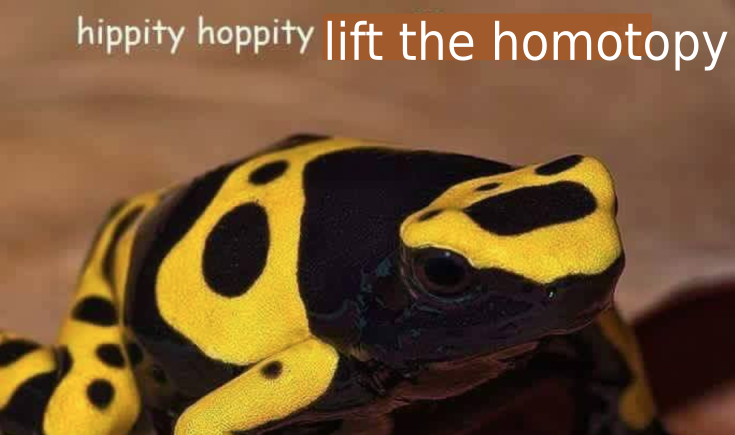
\includegraphics[scale=.22]{pictures/HippityHoppity.png}};
    \end{tikzpicture}
    \pause

    \begin{enumerate}[label=\arabic*)]
	\item Let $z_{0}\in W\subseteq Z$ be an open neighbourhood of a point in $Z$

	    for which there exists a subdivision $0=t_{0}<t_{1}<\cdots <t_{m}=1$

	    such that $p\colon Y\to X$ is trivial over $F(W\times [t_{i},t_{i+1}])$ for all $i$.
	    \pause
	\item Since $p$ is trivial over $F(W\times [0,t_{1}])$, there is a unique way to extend the lifting $\tilde{f}_{0}$ to liftings $\tilde{f}_{t}$ for $t\in [0,t_{1}]$.
	    \pause
	\item Iterate this process to obtain a local lifting $\tilde{F}\colon W\times [0,1]\to Y$.
	    \pause
	\item Do the same for each point $z\in Z$.
	    On the overlaps the extensions agree by ``Maps into covering spaces'' applied to each $\{z\}\times [0,1]$, because $\tilde{F}(z,0)$ has to be $\tilde{f}_{0}(z)$.
    \end{enumerate}
\end{frame}

\begin{frame}
    \frametitle{The monodromy action}
    \begin{figure}[htp]
	\centering
	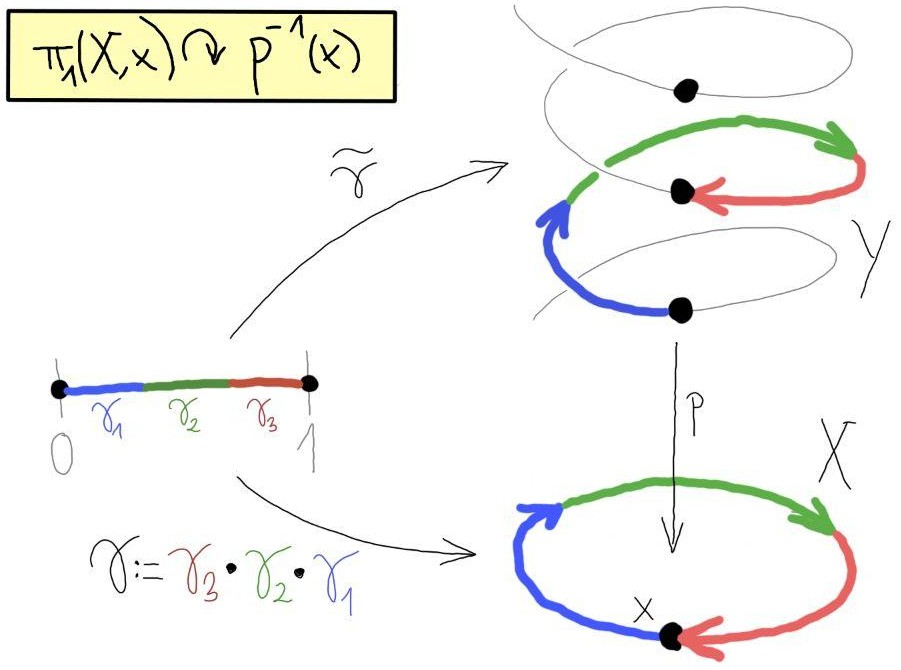
\includegraphics[scale=.25]{pictures/monodromy.jpg}
	\caption{Given the class of a path $[\gamma]\in \pi_{1}(X,x)$ and a point $y\in p^{-1}(x)$, set $[\gamma]\cdot y:=\tilde{\gamma}(1)$, where $\tilde{\gamma}$ is the unique lift of $\gamma$ to the cover.
	Only defining concatenation the unconventional way we obtain a \textit{left} action!}
    \end{figure}
\end{frame}

\begin{frame}
    \frametitle{Cover$\leftrightarrow $Monodromy [$X$ connected+locally $1$-connected]}
    \begin{thm}[{\cite[Theorem 2.3.4]{sza08}}]
	The functor
	\begin{align*}
	    \Fib_{x}\colon \Cov(X) & \longrightarrow \pi_{1}(X,x)-\Set \\
	    (p\colon Y\to X) & \longmapsto \pi_{1}(X,x)\act p^{-1}(x)
	\end{align*}
	is an equivalence of categories from the category of covers of $X$ to the category of sets endowed with a $\pi_{1}(X,x)$-action.
    \end{thm}
    \pause

    \setcounter{exe}{1}
    \begin{exe}
	Check that $\Fib_{x}$ is a functor.
	[Hint: ``Maps into covering spaces''.]
    \end{exe}
\end{frame}

\begin{frame}
    \frametitle{Sketch of proof --- Part 1: the universal cover}
    \begin{enumerate}[label=\arabic*)]
	\item The \textit{universal cover} $\tilde{X}_{x}$ consists of homotopy classes of paths in $X$ starting at $X$, and the projection $\pi\colon \tilde{X}_{x}\to X$ is $\pi([\alpha]):=\alpha(1)$.
	    \pause
	\item Let $y\in p^{-1}(x)$.
	    Define $\pi_{y}\in \Hom_{X}(\tilde{X}_{x},Y)$ by $\pi_{y}([\alpha]):=\tilde{\alpha}(1)$.
	    \pause
	\item Let $\phi\in \Hom_{X}(\tilde{X}_{x},Y)$.
	    Define $y\in p^{-1}(x)$ as $y:=\phi([x])$.
	    \pause
	\item These two maps are mutually inverse, so \framebox{$\Fib_{x}\cong \Hom_{X}(\tilde{X}_{x},-)$}.
	    \pause
	\item $\pi\colon \tilde{X}_{x}\to X$ is Galois, because $\pi_{[\gamma]}$ is an automorphism and $\pi_{[\gamma]}([x])=[\gamma]$ (suffices to check transitivity on a single fibre).
	    \pause
	\item \framebox{$\pi_{1}(X,x)\cong \Aut(\tilde{X}_{x}\mid X)^{\mathrm{op}}$} via $[\gamma]\longmapsto ([\alpha]\mapsto [\alpha\cdot \gamma])$.
	    \pause
	\item Let $\phi\in \Aut(\tilde{X}_{x}\mid X)$ and $y\in p^{-1}(x)$.
	    Define $\phi\cdot y:=\pi_{y}\circ \phi([x])$, i.e.~the point in $\Fib_{x}(Y)$ corresponding to $\pi_{y}\circ \phi\in \Hom_{X}(\tilde{X}_{x},Y)$.
	    Then $\psi\cdot(\phi\cdot y)$ corresponds to $\pi_{y}\circ \phi\circ \psi=\pi_{y}\circ (\psi\circ^{\mathrm{op}}\phi)$.
	    We get $\Aut(\tilde{X}_{x}\mid X)^{\mathrm{op}}\act p^{-1}(x)$, which agrees with $\pi_{1}(X,x)\act p^{-1}(x)$.
    \end{enumerate}
\end{frame}

\begin{frame}
    \frametitle{Sketch of proof --- Part 2: fully faithfulness}
    \begin{enumerate}[label=\arabic*)]
	\item Let $\psi\colon \Fib_{x}(Y)\to \Fib_{x}(Z)$ be $G:=\pi_{1}(X,x)$-equivariant.
	    Want some $f\colon Y\to Z$ over $X$ such that $\psi(y)=f(y)$ for all $y\in p^{-1}(x)$.
	    \pause
	\item We may assume $Y$ and $Z$ connected ($G$-orbits are connected).
	    \pause
	\item Hence faithfulness follows from ``Maps into covering spaces''..
	    \pause
	\item Let $\pi_{y}\colon \tilde{X}_{x}\to Y$ corresponding to $y\in p^{-1}(x)$, so that \framebox{$Y=\Aut(\tilde{X}_{x}\mid Y)\backslash \tilde{X}_{x}$} by Galois correspondence.
	    \pause
	\item Via $G\cong \Aut(\tilde{X}_{x}\mid X)$ we can identify $G_{y}:=\{ g\in G\mid g\cdot y=y\}$ and $\{ \phi\in \Aut(\tilde{X}_{x}\mid X)\mid \pi_{y}\circ \phi =\pi_{y}\}$.
	    Hence \framebox{$\Aut(\tilde{X}_{x}\mid Y)=G_{y}$}.
	    \pause
	\item $G_{y}\subseteq G_{\psi(y)}$ by $G$-equivar.~$\rightsquigarrow f\colon Y=G_{y}\backslash \tilde{X}_{x}\to G_{\psi(y)}\backslash \tilde{X}_{x}=Z$.
	\item $f(y)=f(\pi_{y}([x]))=\pi_{\psi(y)}([x])=\psi(y)$.
	    For $y'\in p^{-1}(y)$, let $\gamma$ s.t.~$[\gamma]\cdot y=y'$, so that $\psi(y')=[\gamma]\cdot \psi(y)$.
	    Then we have
	    \[ f(y')=f\circ\tilde{\gamma}^{Y}(1)=\tilde{\gamma}^{Z}(1)=[\gamma]\cdot \psi(y)=\psi(y'). \]
    \end{enumerate}
\end{frame}

\begin{frame}
    \frametitle{Sketch of proof --- Part 3: essential surjectivity}
    \begin{enumerate}[label=\arabic*)]
	\item Let $S$ be a set with a $G:=\pi_{1}(X,x)$ action.
	    \pause
	\item We may assume $G\act S$ transitive (otherwise split into orbits).
	    \pause
	\item Let $s\in S$ any and let $G_{s}$ be its stabiliser.
	    By Galois correspondence we can find
	    \begin{center}
		\begin{tikzcd}[ampersand replacement=\&]
		    \tilde{X}_{x}\arrow[swap]{dr}{\pi}\arrow{r}{q} \& Y:=G_{s}\backslash \tilde{X}_{x}\arrow{d}{p} \\
		    \& X
		\end{tikzcd}
	    \end{center}
	    \pause
	\item Since $p\colon Y\to X$ is connected, $G\act p^{-1}(x)$ is transitive.
	\item Define $\varphi(q([x])):=s$.
	    We will try to extend by $G$-equivariance.
	    \pause
	\item If $g'\cdot q([x])=g\cdot q([x])$, then $g'g^{-1}\in \Aut(\tilde{X}_{x}\mid Y)=G_{s}$.
	    Hence $\varphi\colon p^{-1}(x) \to S$ defined as $y=g\cdot q([x]) \mapsto g\cdot s$ is $G$-equivar.
	    \pause
	\item If $g\cdot s=g'\cdot s$, then again $g'g^{-1}\in G_{s}=G_{q([x])}$, so $g\cdot q([x])=g'\cdot q([x])$.
	    And transitivity implies surjectivity.
    \end{enumerate}
\end{frame}

\section{Example}
\begin{frame}
    \frametitle{Back to our initial example}
    Let $\pi\colon \C^{\times}\to \C^{\times}$ be our map $z\mapsto z^{2}$, whose fibre over $z_{0}$ consists of the points $\pm\sqrt{z_{0}}$, and let $p\colon Y\to \C^{\times}$ be the cover in which the fibre over $z_{0}\in \C^{\times}$ is the $\Q$-vector space spanned by $\{ \sqrt{z_{0}},-\sqrt{z_{0}}\}$ with the discrete topology\footnote{We can define $p$ formally as the étalé space of the locally constant sheaf $\pi_{*}\Q$.}.
    \pause
    Let $[\gamma]\in \pi_{1}(\C^{\times},1)$ be a generator, say $\gamma(t):=e^{2t\pi i}$.
    We saw at the beginning of the talk that $[\gamma]\cdot \sqrt{1}=-\sqrt{1}$.
    \pause

    Hence the monodromy representation is given by the matrix
    \[ A:=\begin{pmatrix}
	0 & 1 \\
	1 & 0
    \end{pmatrix},
    \]
    meaning that $\pi_{1}(\C^{\times},1)\to \operatorname{GL_{2}(\Q)}$ maps $[\gamma]$ to $A$.
    \pause
    \begin{exe}
	A \normalfont{subrepresentation} of $\rho\colon G\to \operatorname{GL}(V)$ consists of a $G$-invariant subspace $W\subseteq V$ together with the induced $G\to \operatorname{GL}(W)$.
	Find all subrepresentations of this monodromy action.
	What are the fibres at a point $z_{0}\in \C^{\times}$ of the corresponding covering spaces?
    \end{exe}
\end{frame}

\begin{frame}
    \frametitle{Thanks for your attention!}
    Main reference:
    \bibliographystyle{alpha}
    \bibliography{main.bib}
\end{frame}

\end{document}
